\documentclass[submission]{eptcs}
\providecommand{\event}{TTC 2015}

\usepackage[T1]{fontenc}
\usepackage{varioref}
\usepackage{hyperref}

\usepackage{url}
\usepackage{paralist}
\usepackage{graphicx}
\usepackage[cache]{minted}
\newminted{clojure}{fontsize=\fontsize{8}{8},linenos,numbersep=3pt,numberblanklines=false}
\newmintinline{clojure}{fontsize=\small}
\newcommand{\code}{\clojureinline}
\VerbatimFootnotes

\title{Solving the TTC Train Benchmark Case with FunnyQT}
\author{Tassilo Horn
  \institute{Institute for Software Technology, University Koblenz-Landau, Germany}
  \email{horn@uni-koblenz.de}}

\def\titlerunning{Solving the TTC Train Benchmark Case with FunnyQT}
\def\authorrunning{T. Horn}

\begin{document}
\maketitle

\begin{abstract}
  This paper describes the FunnyQT solution to the TTC 2015 Train Benchmark
  transformation case.  The solution solves all core and all extension tasks.
  FunnyQT is a model querying and model transformation library for the
  functional Lisp-dialect Clojure providing a comprehensive and efficient
  querying and transformation API, many parts of which are provided as
  task-oriented embedded DSLs.
\end{abstract}


\section{Introduction}
\label{sec:introduction}

This paper describes the FunnyQT\footnote{\url{http://funnyqt.org}}
~\cite{Horn2013MQWFQ,funnyqt-icgt15} solution of the TTC 2015 Train Benchmark
Case~\cite{train-benchmark-case-desc}.  All core and extension tasks have been
solved.  The solution project is available on
Github\footnote{\url{https://github.com/tsdh/ttc15-train-benchmark-funnyqt}},
and it is set up for easy reproduction on a SHARE image\footnote{The SHARE
  image name is \verb|ArchLinux64_TTC15-FunnyQT|}.

FunnyQT is a model querying and transformation library for the functional Lisp
dialect Clojure\footnote{\url{http://clojure.org}}.  Queries and
transformations are plain Clojure programs using the features provided by the
FunnyQT API.

As a Lisp, Clojure provides strong metaprogramming capabilities that are
exploited by FunnyQT in order to define several \emph{embedded domain-specific
  languages} (DSL, \cite{book:Fowler2010DSL}) for different querying and
transformation tasks.

FunnyQT is designed with extensibility in mind.  By default, it supports EMF
\cite{Steinberg2008EEM} models and
JGraLab\footnote{\url{http://jgralab.github.io}} TGraph models.  Support for
other modeling frameworks can be added without having to touch FunnyQT's
internals.

The FunnyQT API is structured into the following namespaces, each namespace
providing constructs supporting concrete querying and transformation use-cases:

\begin{compactdesc}
\item[funnyqt.emf] EMF-specific model management API
\item[funnyqt.tg] JGraLab/TGraph-specific model management API
\item[funnyqt.generic] Protocol-based, generic model management API
\item[funnyqt.query] Generic querying constructs such as quantified expressions
  or regular path expressions
\item[funnyqt.polyfns] Constructs for defining polymorphic functions
  dispatching on metamodel types
\item[funnyqt.pmatch] Pattern matching constructs
\item[funnyqt.relational] Constructs for logic-based, relational model querying
  inspired by Prolog
\item[funnyqt.in-place] In-place transformation rule definition constructs
\item[funnyqt.model2model] Out-place transformation definition constructs
  similar to ATL or QVT Operational Mappings
\item[funnyqt.extensional] Transformation API similar to GReTL
\item[funnyqt.bidi] Constructs for defining bidirectional transformations
  similar to QVT Relations
\item[funnyqt.coevo] Constructs for transformations that evolve a metamodel and
  a conforming model simultaneously at runtime
\item[funnyqt.visualization] Model visualization
\item[funnyqt.xmltg] Constructs for querying and modifying XML files as models
  conforming to a DOM-like metamodel
\end{compactdesc}

For solving the train benchmark case, the \emph{funnyqt.emf} and
\emph{funnyqt.in-place} namespaces have been used.


\section{Solution Description}
\label{sec:solution-description}

In this section, the individual tasks are discussed one by one.  They are all
implemented as in-place transformation rules supported by FunnyQT's
\emph{funnyqt.in-place} transformation DSL.  The rules' repair actions simply
call the CRUD functions of the EMF-specific \emph{funnyqt.emf} namespace.

\paragraph{Task 1: PosLength.}

The transformation rule realizing the \emph{PosLength} task is given below.

\begin{clojurecode}
(defrule pos-length {:forall true :recheck true} [g]
  [segment<Segment>
   :when (<= (eget-raw segment :length) 0)]
  (eset! segment :length (inc (- (eget-raw segment :length)))))
\end{clojurecode}

The \code|defrule| macro defines a new in-place transformation rule with the
given name (\code|pos-length|), an optional map of options
(\code|{:forall true, ...}|) a vector of formal parameters (\code|[g]|), a
pattern (\code|[segment<Segment>...]|), and one or many actions to be applied
to the pattern's matches (\code|(eset! ...)|).  The first formal parameter must
denote the model the rule is applied to, so here the argument \code|g| denotes
the train model when the rule is applied using
\code|(pos-length my-train-model)|.

The pattern matches a node called \code|segment| of metamodel class
\code|Segment|.  Additionally, the segment's length must be less or equal to
zero as defined by the \code|:when| constraint.  The action says that the
segment's \code|length| attribute should be set to the incremented negation of
the current length.

The normal semantics of applying a rule is to find one single match of the
rule's pattern and then execute the rule's actions on the matched elements.
The \code|:forall| option changes this behavior to finding all matches first,
and then applying the actions to each match one after the other.  FunnyQT
automatically parallelizes the pattern matching process of such forall-rules
under certain circumstances like the JVM having more than one CPU available and
the pattern declaring at least two elements to be matched.

The \code|:recheck| option causes the rule to recheck if a pre-calculated match
is still conforming the pattern just before executing the rule's actions on it.
This can be needed for forall-rules whose actions possibly invalidate matches
of the same rule's pattern, e.g., when the application of the action to a match
\(m_i\)
cause another match \(m_j\)
to be no valid match any longer\footnote{This cannot happen for the
  \code|pos-length| rule, however the case description demands matches to be
  revalidated before applying the repair actions.}.


\paragraph{Task 2: SwitchSensor.}

The transformation rule realizing the \emph{SwitchSensor} task is given below.

\begin{clojurecode*}{firstnumber=last}
(defrule switch-sensor {:forall true :recheck true} [g]
  [sw<Switch> -!<:sensor>-> <>]
  (eset! sw :sensor (ecreate! nil 'Sensor)))
\end{clojurecode*}

It matches a switch \code|sw| which is not contained by some sensor.  The
exclamation mark of the edge symbol \code|-!<:sensor>->| specifies that no such
reference must exist, i.e., it specifies a negative application condition.  The
action fixes this problem by creating a new \code|Sensor| and assigning that to
the switch \code|sw|.


\paragraph{Task 3: SwitchSet.}

The \code|switch-set| rule realizes the \emph{SwitchSet} task.  Its definition
is given below.

\begin{clojurecode*}{firstnumber=last}
(def Signal-GO (eenum-literal 'Signal.GO))

(defrule switch-set {:forall true :recheck true} [g]
  [route<Route> -<:entry>-> semaphore
   :when (= (eget-raw semaphore :signal) Signal-GO)
   route -<:follows>-> swp -<:switch>-> sw
   :let [swp-pos (eget-raw swp :position)]
   :when (not= (eget-raw sw :currentPosition) swp-pos)]
  (eset! sw :currentPosition swp-pos))
\end{clojurecode*}

It matches a \code|route| with its entry \code|semaphore| where the semaphore's
signal is \code|Signal.GO|.  The route follows some switch position \code|swp|
whose switch \code|sw|'s current position is different from that of the switch
position.  The fix is to set the switch's current position to the position of
the switch position \code|swp|.

Note that there are no metamodel types specified for the elements
\code|semaphore|, \code|swp|, and \code|sw| because those are already defined
implicitly by the references leading to them, e.g., all elements referenced by
a route's \code|follows| reference can only be instances of
\code|SwitchPosition| according to the metamodel.  FunnyQT doesn't require the
transformation writer to encode tautologies in her patterns\footnote{In fact,
  if there are types specified, those will be checked.  So omitting them when
  they are not needed also results in slightly faster patterns.}.


\paragraph{Extension Task 1: RouteSensor.}

The extension task \emph{RouteSensor} is realized by the \code|route-sensor|
rule given below.

\begin{clojurecode*}{firstnumber=last}
(defrule route-sensor {:forall true :recheck true} [g]
  [route<Route> -<:follows>-> swp -<:switch>-> sw
   -<:sensor>-> sensor --!<> route]
  (eadd! route :definedBy sensor))
\end{clojurecode*}

It matches a \code|route| that follows some switch position \code|swp| whose
switch \code|sw|'s \code|sensor| is not contained by the \code|route|.  The
repair action is to assign the \code|sensor| to the \code|route|.


\paragraph{Extension Task 2: SemaphoreNeighbor.}

The second and last extension task \emph{SemaphoreNeighbor} is realized by the
\code|semaphore-neighbor| rule defined as shown below.

\begin{clojurecode*}{firstnumber=last}
(defrule semaphore-neighbor {:forall true :recheck true} [g]
  [route1<Route> -<:exit>-> semaphore
   route1 -<:definedBy>-> sensor1 -<:elements>-> te1
   -<:connectsTo>-> te2 -<:sensor>-> sensor2
   --<> route2<Route> -!<:entry>-> semaphore
   :when (not= route1 route2)]
  (eset! route2 :entry semaphore))
\end{clojurecode*}

It matches a route \code|route1| which has an exit \code|semaphore|.
Additionally, \code|route1| is defined by a sensor \code|sensor1| which
contains some track element \code|te1| that connects to some track element
\code|te2| whose sensor is \code|sensor2|.  This \code|sensor2| is contained by
some other route \code|route2| which does not have \code|semaphore| as entry
semaphore.  The fix is to set \code|route2|'s entry reference to
\code|semaphore|.


\subsection{Deferred Rule Actions}
\label{sec:deferred-actions}

As already mentioned above, the normal semantics of a forall-rule is to compute
all matches of the rule's pattern first (possibly in parallel), and then apply
the rule's actions on every match one after the other.  However, the case
description strictly separates the computation of matches from the repair
transformations.

FunnyQT also provides stand-alone patterns.  Using them, one could have defined
patterns for finding occurrences of the five problematic situations in a train
model, and separate functions for the repair actions where the latter receive
one match of the corresponding pattern and fix that.

But for in-place transformation rules, FunnyQT also provides \emph{rule
  application modifiers}.  Concretely, any in-place transformation rule
\code|r| can be called as \code|(as-pattern (r model))| in which case it
behaves as a pattern.  That is, where a normal rule would usually find one
match and apply its actions on it and a forall-rule would usually find all
matches and apply its actions to each of them, when called with
\code|as-pattern|, a rule simply returns the sequence of its matches.  With a
normal rule, this sequence is a lazy sequence, i.e., the matches are not
computed until they are consumed.  With a forall-rule, the sequence is fully
realized, i.e., all matches are already pre-calculated (possibly in parallel).

The second FunnyQT rule application modifier is \code|as-test|, and this is
what is highly suitable for this transformation case.  When a rule \code|r| is
applied using \code|(as-test (r model))|, it behaves almost as without modifier
but instead of applying the rule's actions immediately, it returns a closure of
arity zero (a so-called \emph{thunk}) which captures the rule's match and the
rule's actions.  Invoking the thunk causes the actions to be applied on the
match.  Thus, the caller of the rule gets the information if the rule was
applicable at all, and if it was applicable, she can decide if she wants to
apply it or not.  And when she applies it, the pattern matching part is already
finished and only the actions are applied on the pre-calculated match the thunk
closes over.  The following snippet illustrates the behavior.

\begin{clojurecode*}{numbers=none}
(if-let [thunk (as-test (r model))]
  (if (< (Math/random) 0.5)
    (thunk) ;; The rule was applicable, and here its actions are executed
    (println "The coin toss decided to skip the application of the rule's actions"))
  (println "The rule is not applicable"))
\end{clojurecode*}

One interesting point is that the thunk returned by calling a rule as a test
has some metadata attached\footnote{Almost any Clojure object (functions,
  symbols, vars, collections, etc.) can have metadata attached.  Metadata
  doesn't affect equality, i.e., two Clojure objects that differ only in their
  metadata are still equal.}.  For this TTC case, only the \code|:match|
metadata entry is important.  As its name suggests, its value is the match of
the rule's pattern on which the thunk applies the actions.

In case of a forall-rule \code|r|, \code|(as-test (r model))| doesn't return a
single thunk but a vector of thunks, one thunk per match of the rule's pattern.
This is exactly what is needed for solving this transformation case.

Finally, a function is defined that receives a rule \code|r| and a train model
\code|g| and executes the rule as a test.

\begin{clojurecode*}{firstnumber=27}
(defn call-rule-as-test [r g]
  (as-test (r g)))
\end{clojurecode*}

This is only needed in order to be able to call the rules as tests from Java.
The reason is that only functions (and rules which are functions, too) can be
referred to from Java but \code|as-test| is a macro which does its magic at
compile-time.

These 28 lines of Clojure code form the complete functional part of the FunnyQT
solution that solves all core and extension tasks.  The comparator used for
sorting the matches in the benchmark framework is also implemented using
Clojure/FunnyQT and discussed in section~\vref{sec:match-comparison}.
Additionally, there is a plain-Java glue project which implements the
interfaces required by the benchmark framework and simply delegates to the
Clojure/FunnyQT part of the solution.  This glue project is briefly discussed
in section~\vref{sec:gluing}.


\subsection{Match Comparison}
\label{sec:match-comparison}

The case description demands that solutions provide comparators that are to be
used for sorting matches.  All comparators simply compare two matches element
by element with respect to the values of the \textsf{id}-attribute.  The order
in which the elements of two matches have to be compared is defined separately
for each task.

Instead of providing one comparator per task, the FunnyQT solution provides one
higher-order function \code|make-match-comparator| which receives the names of
the match elements to be compared and then returns a suitable comparator.  The
function's definition is given below.

\begin{clojurecode}
(defn make-match-comparator [& kws]
  (fn [t1 t2]
    (loop [kws kws]
      (if (seq kws)
        (let [m1 ((first kws) (:match (meta t1)))
              m2 ((first kws) (:match (meta t2)))]
          (let [r (compare (eget m1 :id) (eget m2 :id))]
            (if (zero? r)
              (recur (rest kws))
              r)))
        0))))
\end{clojurecode}

The \code|make-match-comparator| function is to be used as follows.

\begin{clojurecode*}{numbers=none}
(make-match-comparator :segment)
;=> comparator for pos-length
(make-match-comparator :sw)
;=> comparator for switch-sensor
(make-match-comparator :semaphore :route :swp :sw)
;=> comparator for switch-set
(make-match-comparator :route :sensor :swp :sw)
;=> comparator for route-sensor
(make-match-comparator :semaphore :route1 :route2 :sensor1 :sensor2 :te1 :te2)
;=> comparator for semaphore-neighbor
\end{clojurecode*}


\code|make-match-comparator| returns a function of two arguments.  In Clojure,
every function implements the \code|java.util.Comparator| interface and thus
any function of two arguments which returns an integer can be used as such.

The returned comparator function receives two thunks \code|t1| and \code|t2|
that where returned by calling any of the five above rules as tests.  Then it
iterates the keywords denoting the matched element names.  Lines 5 and 6
extract the actual elements of the thunks' matches which are denoted by the
first keyword.  Then line 7 compares the \textsf{id} attribute values.  If the
comparison returns a non-zero value and thus these elements are different, the
value is simply returned.  Otherwise, the remaining keywords are tested one
after the other.  Only if no distinction between matches can be made after
considering all given keywords, zero is returned.



\subsection{Gluing the Solution with the Framework}
\label{sec:gluing}

Typically, open-source Clojure libraries and programs are distributed as JAR
files that contain the source files rather than byte-compiled class files.
This solution does the same, and that JAR is deployed to a local Maven
repository from which the Maven build infrastructure of the benchmark framework
can pick it up.

Then, in the FunnyQT glue project the rules and functions from above are
referred to like shown in the next listing.

\begin{minted}[fontsize=\fontsize{8}{8},linenos,numbersep=3pt,numberblanklines=false]{java}
private final static String SOLUTION_NS = "ttc15-train-benchmark-funnyqt.core";
Clojure.var("clojure.core", "require").invoke(Clojure.read(SOLUTION_NS));
final static IFn POS_LENGTH = Clojure.var(SOLUTION_NS, "pos-length");
...
final static IFn CALL_RULE_AS_TEST = Clojure.var(SOLUTION_NS, "call-rule-as-test");
\end{minted}

In line 2, the solution namespace \code|ttc15-train-benchmark-funnyqt.core| is
required\footnote{\code|require| is kind of Clojure's equivalent to Java's
  \code|import| statement.}.  The \code|Clojure| class provides a minimal API
for loading Clojure code from Java.  When requiring a namespace as above, it
will be parsed and compiled to JVM byte-code just in time\footnote{If the
  Clojure code was distributed in a pre-compiled form, the resulting classes
  would simply be loaded.}.

Thereafter, the solution's in-place transformation rules and the
\code|call-rule-as-test| function are referred to.  \code|IFn| is a Clojure
interface whose instances are Clojure functions that can be called using the
\code|invoke()| method as can be seen in the definition of the glue project's
\code|BenchmarkCase.check()| method shown below.

\begin{minted}[fontsize=\fontsize{8}{8},linenos,numbersep=3pt,numberblanklines=false]{java}
@Override
protected final Collection<Object> check() throws IOException {
    matches = (Collection<Object>) FunnyQTBenchmarkLogic.CALL_RULE_AS_TEST
                                   .invoke(rule, this.resource);
    // If the rule has no matches it returns nil/null but the framework
    // wants a Collection.
    if (matches == null) {
        matches = new LinkedList<Object>();
    }
    return matches;
}
\end{minted}

In that code, \code|rule| is one of the rule \code|IFn|s \code|POS_LENGTH|,
\code|SWITCH_SET|, et cetera, and they are called via the
\code|call-rule-as-test| function to make them return one thunk per match
instead of performing the rules' repair actions immediately.

The implementation of the \code|BenchmarkCase.modify()| method is even simpler.

\begin{minted}[fontsize=\fontsize{8}{8},linenos,numbersep=3pt,numberblanklines=false]{java}
@Override
protected final void modify(Collection<Object> matches) {
    for (Object m : matches) {
        ((IFn) m).invoke();
    }
}
\end{minted}

Since the rules are called as tests and thus return thunks that apply the
rule's actions, those simply need to be invoked, and that's it.



\section{Evaluation}
\label{sec:evaluation}

\paragraph{Correctness and Completeness.}

The FunnyQT solution implements all core and all extension tasks exactly as
demanded by the case description, thus it is complete.  When run in the
benchmark framework, all assertion it checks are satisfied, thus the solution
is also correct.

According to the case description, this gives a \emph{correctness and
  completeness score} of 15 points.

\paragraph{Conciseness.}

The FunnyQT solution consists of 28 NCLOC of FunnyQT/Clojure code for the five
rules with their patterns and repair actions, and the function
\code|call-rule-as-test|.

In comparison, the reference EMF-IncQuery solution has about 70 NCLOC only for
the patterns plus 69 NCLOC of plain Java code for the repair actions.
Honestly, more than half of the lines of the Java repair actions are
boilerplate code.  So by a fair measure one could say that the EMF-IncQuery
solution consists of a little bit less than 100 lines of code which actually
implement the solution and are no boilerplate.

The reference Java solution consists of 305 NCLOC for the queries and repair
actions (excluding the classes for the custom match representations).  On the
one hand, one could subtract maybe 10\% for boilerplate code but on the other
hand, when encoding queries and transformations in Java, boilerplate code is a
fact you have to live with.

To sum up, the FunnyQT solution is about three times shorter than the
EMF-IncQuery solution and about ten times shorter than the Java solution.
Thus, if there is no even more concise solution, it deserves a
\emph{conciseness score} of 15 points.

\paragraph{Readability.}

Readability is a very subjective matter, of course, so I won't suggest a
\emph{readability score} value here.  However, there are some strong points
with respect to readability.

\begin{compactitem}
\item The queries (patterns) and repair actions are bundled in one concise
  in-place transformation rule each.  In contrast, in the EMF-IncQuery as well
  as the Java solution the queries and repair transformations are strictly
  separated.  But the latter still depend on the former in that they can only
  work with the matches produced by the former.
\item FunnyQT's pattern matching DSL used to specify the rules' patterns is
  both concise and readable.  It should be easy to understand for graph
  transformation experts, especially if they have used other textual graph
  transformation languages such as \emph{GrGen.NET} before.  It should also be
  easy to understand for any Clojure programmer because it strictly conforms to
  the style guidelines and best practices there, too.
\end{compactitem}

\paragraph{Performance.}

Figure~\Vref{fig:performance-fixed} and Figure~\vref{fig:performance-prop} show
the runtimes of the FunnyQT solution for all models up to the size of 8192
(12,512,663 elements, 23,048,272 references) and the fixed and proportional
strategies as measured by the train benchmark framework.  The tests have been
performed on an 2.7 GHz 8-core machine with 16 GB of RAM being dedicated to the
JVM process.

\begin{figure}[h!tb]
  \centering
  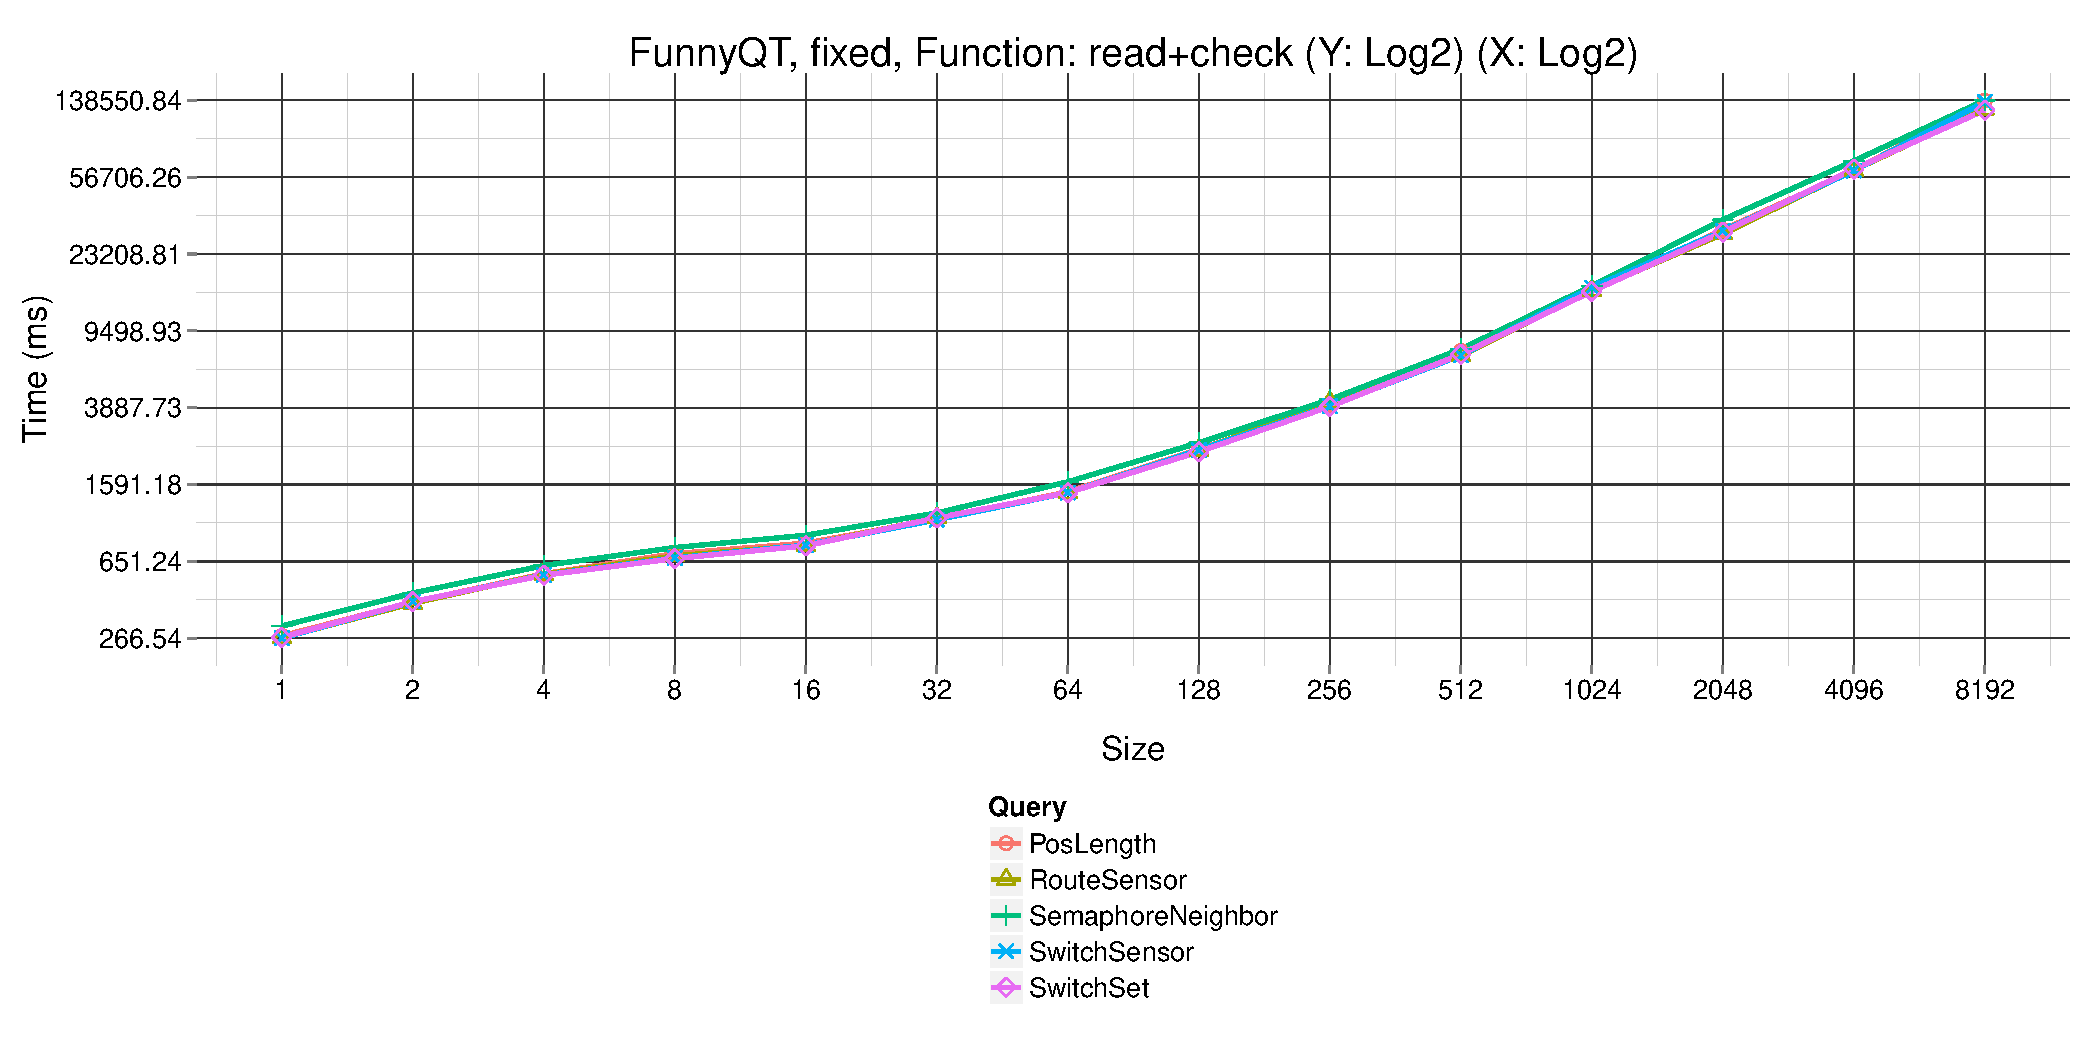
\includegraphics[width=\textwidth]{perf/fixed-FunnyQT-GroupBy-Query-time-batch-validation}

  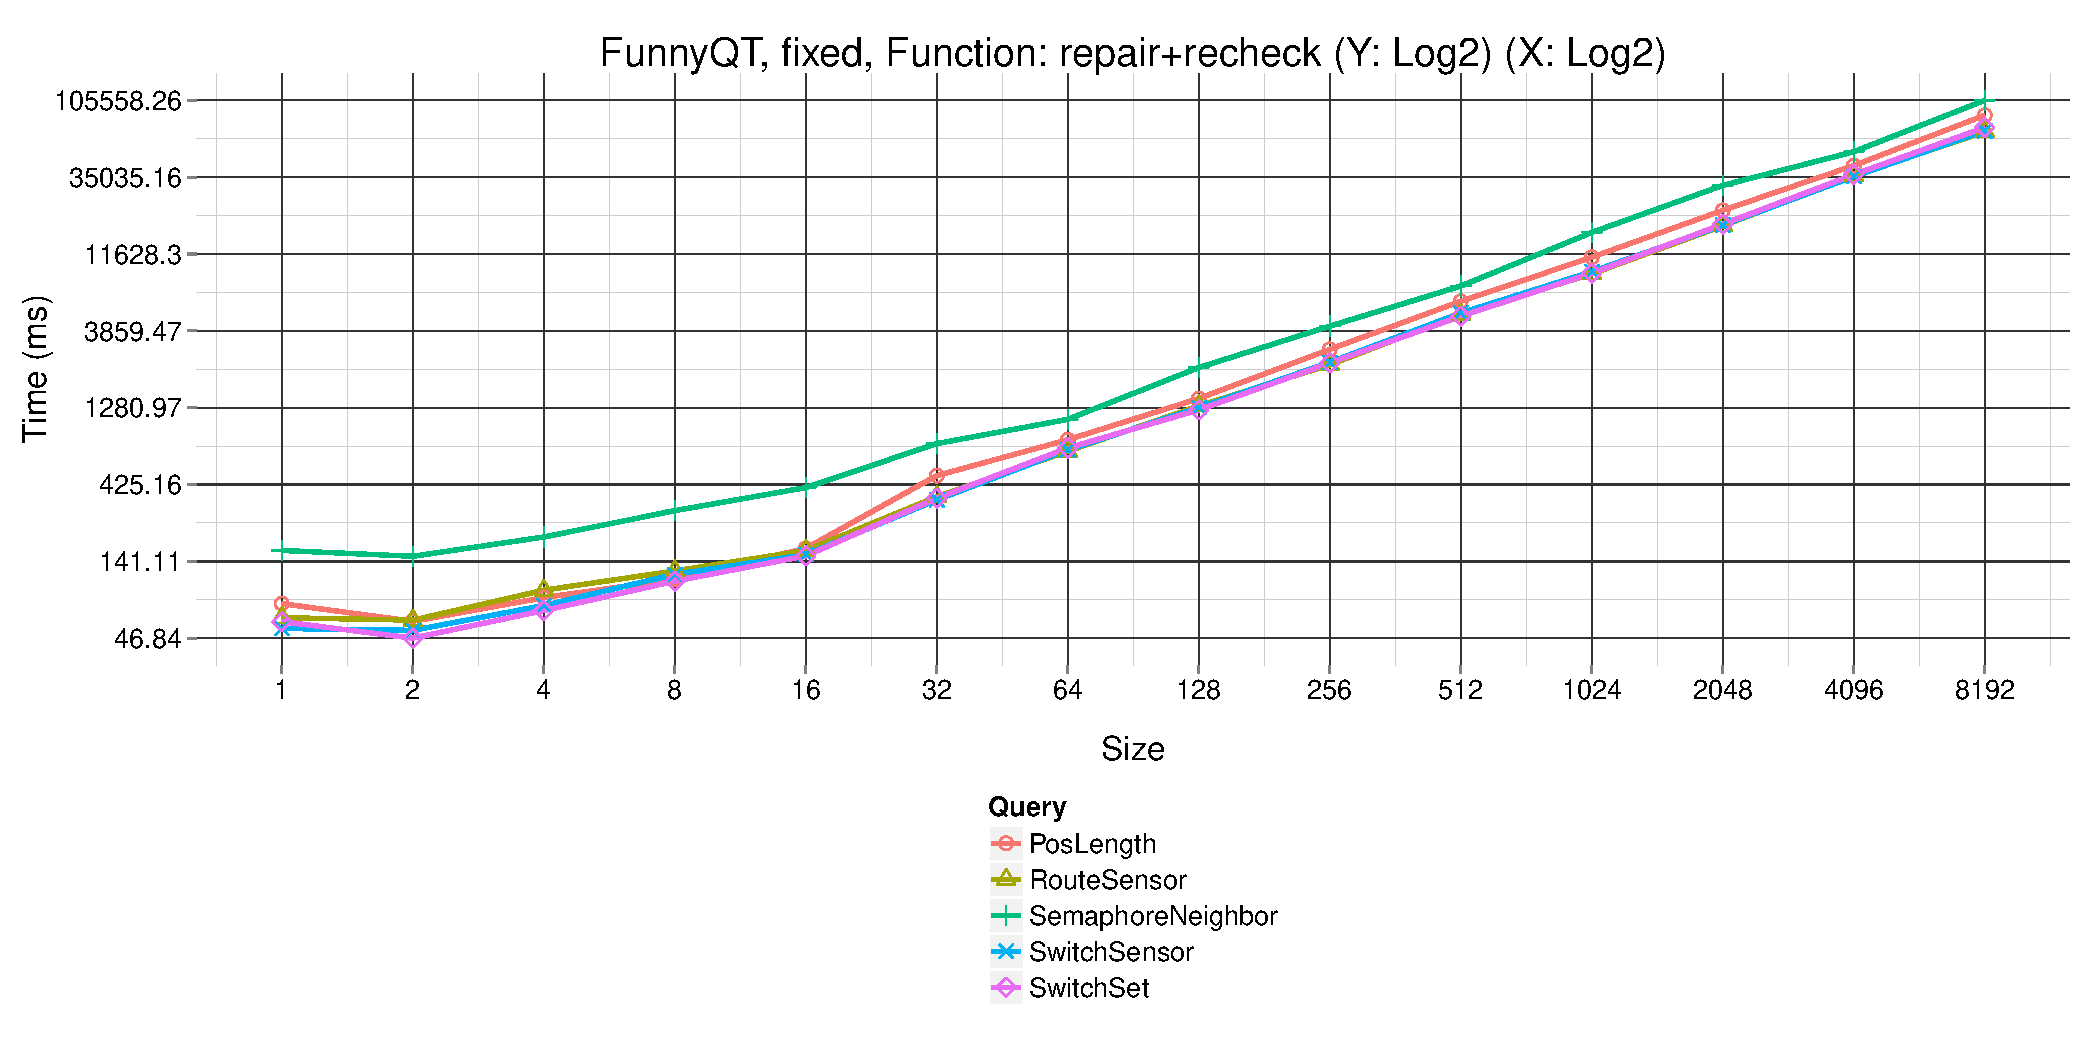
\includegraphics[width=\textwidth]{perf/fixed-FunnyQT-GroupBy-Query-time-revalidation}
  \caption{Results of the performance measurements (\emph{fixed} strategy)}
  \label{fig:performance-fixed}
\end{figure}

\begin{figure}[h!tb]
  \centering
  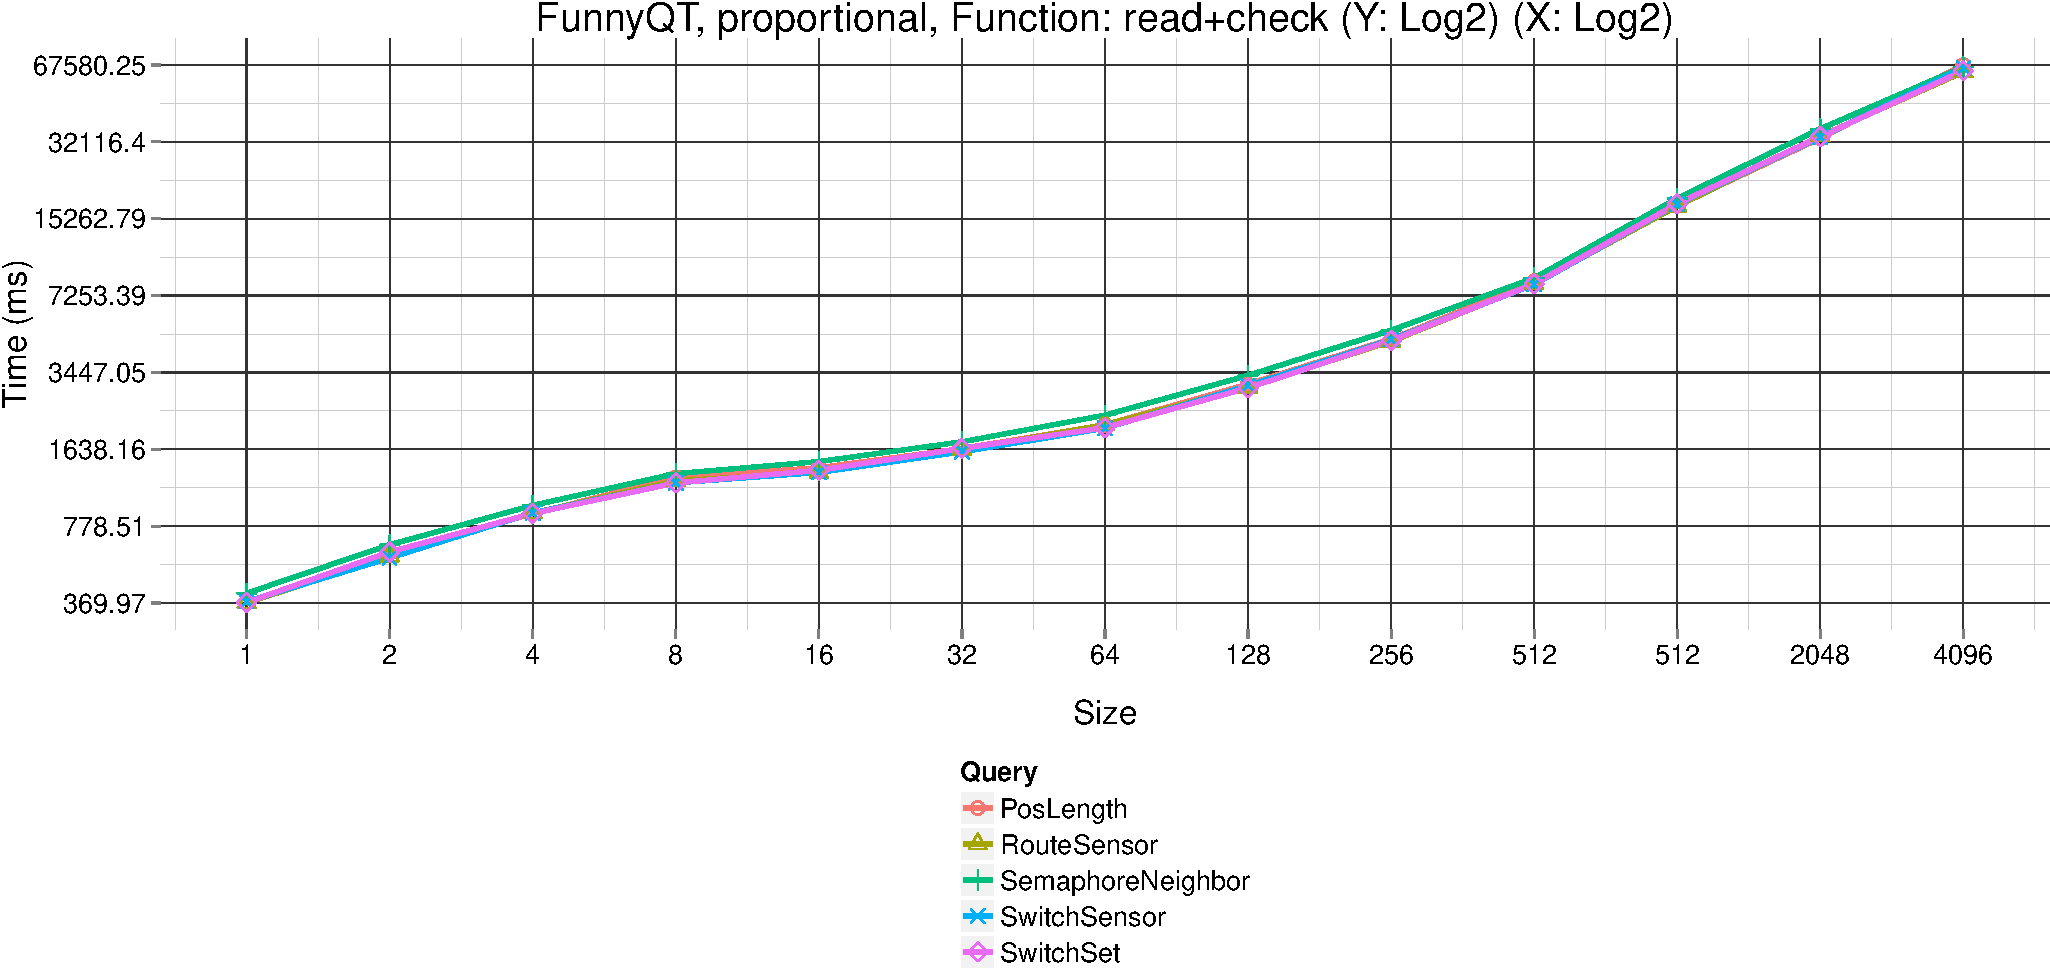
\includegraphics[width=\textwidth]{perf/proportional-FunnyQT-GroupBy-Query-time-batch-validation}

  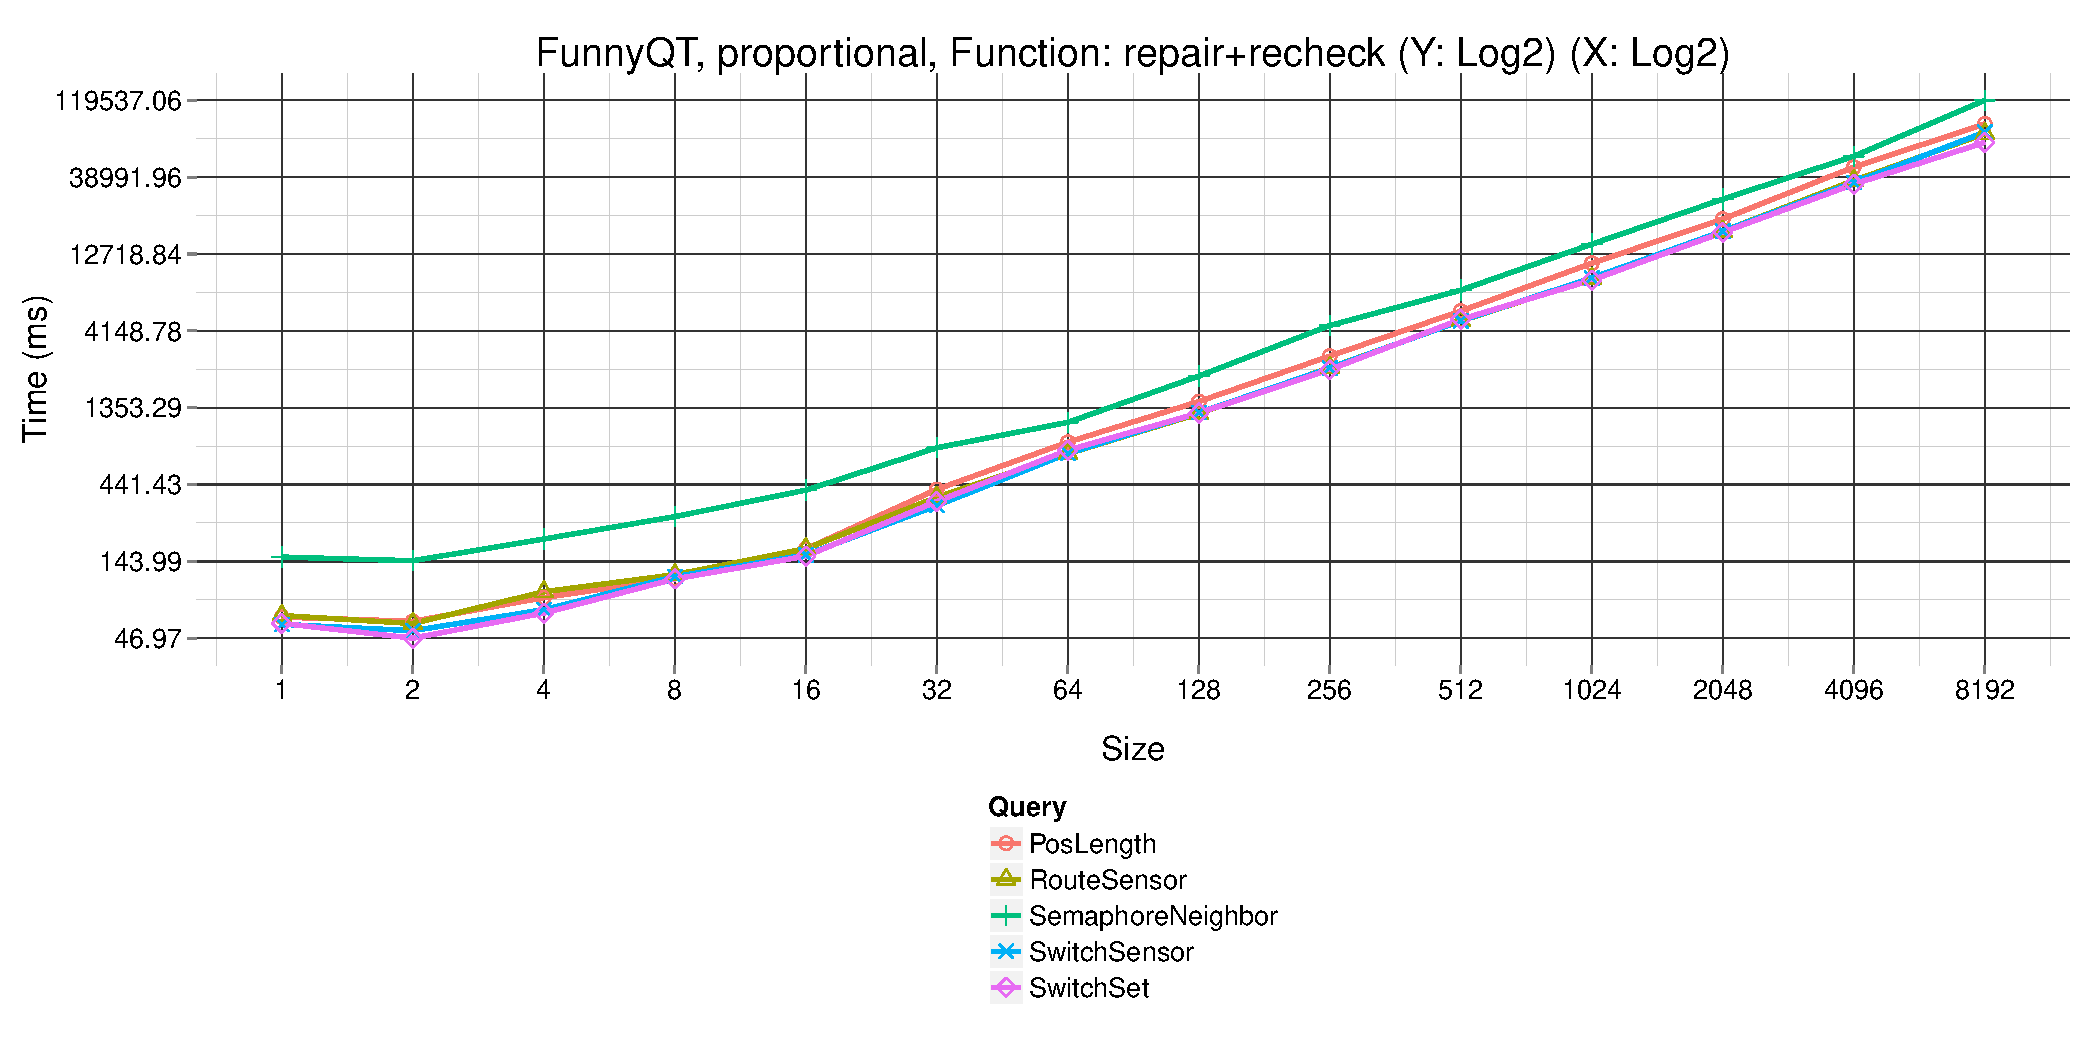
\includegraphics[width=\textwidth]{perf/proportional-FunnyQT-GroupBy-Query-time-revalidation}
  \caption{Results of the performance measurements (\emph{proportional} strategy)}
  \label{fig:performance-prop}
\end{figure}

For the most complex rule \code|semaphore-neighbor| and the largest model with
over twelve million elements, the initial \emph{read \& check} phase takes
slightly less than 140 seconds for both the fixed and the proportional
strategies.  Almost all of this time is spend for loading the model.

The 10 iterations of the \emph{repair \& recheck} phase take about 100 seconds
for both the fixed and proportional strategies, i.e., every iteration is
performed in about 10 seconds.

The benchmarks have also be run for the reference Java and the EMF-IncQuery
solution on the same test machine.  For the Java solution, the initial
\emph{read \& check} phase is slightly faster than the FunnyQT solution but the
10 iterations of the \emph{repair \& recheck} phase only take 64 seconds which
is astonishing.  Of course, a general pattern matching approach like that of
FunnyQT has some overhead when compared to a hand-crafted algorithm.  But the
iteration order implied by the FunnyQT pattern equals that of the Java
solution, and the FunnyQT solution performs the search in parallel on all 8 CPU
cores.  The only obvious differences between the FunnyQT solution and the Java
solution is that the former rechecks matched elements before applying the
repair actions whereas the latter doesn't.  However, the rechecking only
accounts for a tiny fraction of the overall execution time and thus doesn't
explain the execution time difference.

When compared with the EMF-IncQuery solution one can say that the FunnyQT
solution performs better in the scenarios defined by the case description.
With 16 GB of memory dedicated to the JVM process, the EMF-IncQuery
\emph{SemaphoreNeighbor} query fails for the model of size of 8192.  When
comparing the overall execution time for the model of size 4096, i.e., the sum
of the \emph{read \& check} and the 10 iterations of the \emph{repair \&
  recheck} phase, the FunnyQT solution is also a bit faster than the
EMF-IncQuery solution.  However, with the incremental pattern matching approach
of EMF-IncQuery, the \emph{repair \& recheck} phase is extremely fast.  Thus,
when increasing the iteration count from 10 to some higher value, the
EMF-IncQuery solution will eventually outperform the FunnyQT solution pretty
easily.

One thing to note is that the FunnyQT solution is about 20-30\% faster when it
is run in its stand-alone project instead of being invoked by the train
benchmark framework.  The reason for this fact is unknown.



\section{Conclusion}
\label{sec:conclusion}

This paper described the FunnyQT solution to the TTC 2015 Train Benchmark case.
It solves all three core tasks and all two extension tasks, and the benchmark
framework provides evidence that it delivers correct results.

The solution is extremely concise.  Its five rules and one function amount to a
total of only 28 lines of code (excluding comments, empty lines, and namespace
declarations\footnote{Namspace declarations are Clojure's equivalent to Java's
  \mintinline{java}|package| and \mintinline{java}|import| statements.}).

With respect to readability, FunnyQT's pattern matching/in-place transformation
rule DSL should be quite familiar to both people with a graph transformation
background and people with a Clojure background.  A strong point is that the
patterns matching invalid subgraphs and the corresponding repair actions are
defined in one place as transformation rules.  Nevertheless, the matching part
and the application of the repair actions on (only parts of) the matches is
well-supported using FunnyQT's rule application modifier macro \code|as-test|.

The FunnyQT solution also performs very well for large models although the
incremental pattern matching approach inherent to the EMF-IncQuery solution can
easily outperform the FunnyQT solution when increasing the iteration count of
the \emph{repair \& recheck} phase from 10 iterations to 20 or more.  Like with
all traditional, search-based pattern matching approaches, FunnyQT's prime
scenario isn't the incremental one.  If one would measure the time needed for
finding all invalid subgraphs and repairing them all at once, then FunnyQT is a
very competitive approach due to its feature of performing parallel pattern
matching automatically for forall-rules on multi-core machines.  In scenarios
where rules should find just one match and perform actions on that, FunnyQT's
normal rules that perform lazy pattern matching also achieve a very high
performance.

Another aspect speaking in favor of FunnyQT is its comprehensiveness.  Next to
the pattern matching and in-place transformation constructs used for solving
this TTC case, it provides APIs and embedded DSLs suitable for solving almost
any conceivable querying and transformation tasks.


\bibliographystyle{eptcs}
\bibliography{ttc-train-benchmark}
\end{document}

%%% Local Variables:
%%% mode: latex
%%% TeX-master: t
%%% TeX-command-extra-options: "-shell-escape"
%%% LaTeX-verbatim-macros-with-delims-local: ("code")
%%% End:

%  LocalWords:  parallelizes
